\printbibliography
\newpage

\appendix
\noindent
\twocolumn
\section{Segmentation Models}

\begin{figure}[h]
	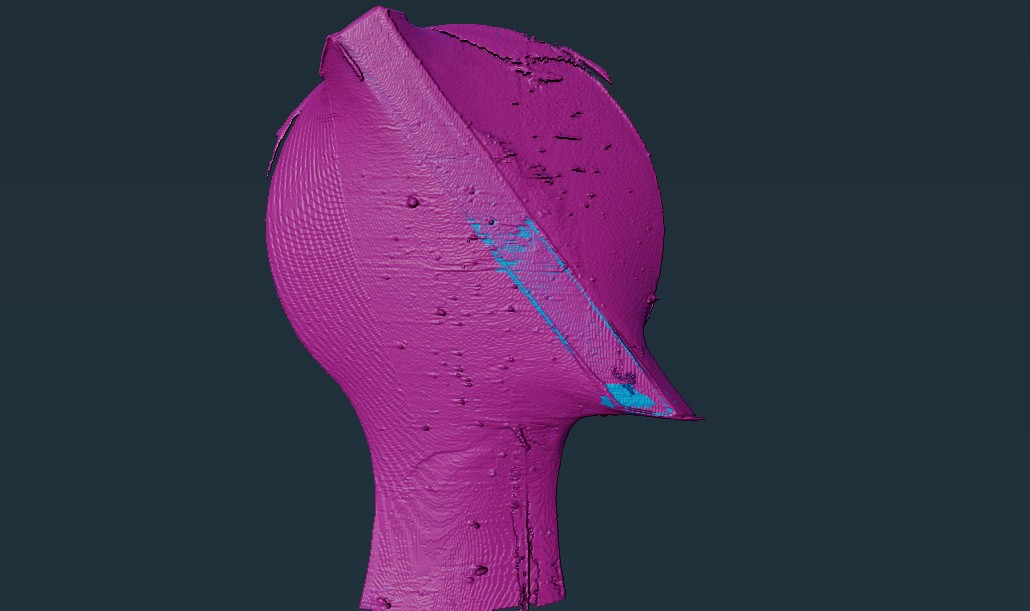
\includegraphics[width=0.5\textwidth]{images/avizo_flats/tlys_9.jpg}
	\caption{Volume rendering in Avizo:\ac{t1} crystal}
 \label{tlys9}
\end{figure}
\begin{figure}
	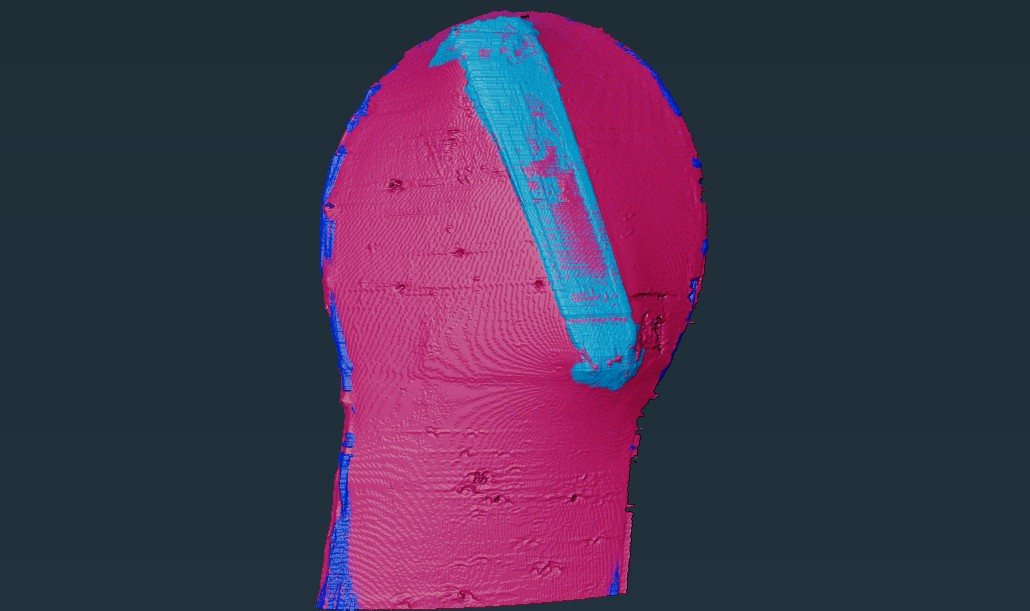
\includegraphics[width=0.5\textwidth]{images/avizo_flats/tlys2.jpg}
	\caption{Volume rendering in Avizo: \ac{t2} crystal}
 \label{tlys2}
\end{figure}
%\begin{figure}
	%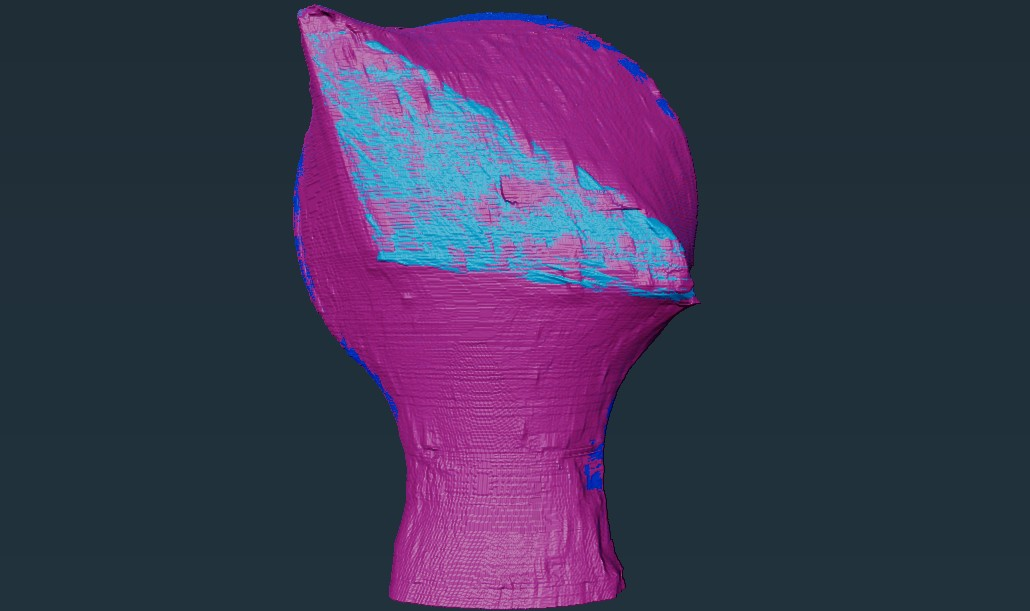
\includegraphics[width=0.5\textwidth]{images/avizo_flats/cas3_1118.jpg}
	%\caption{Volume rendering in Avizo:}
%\label{cas3}
%\end{figure}



\begin{figure}
	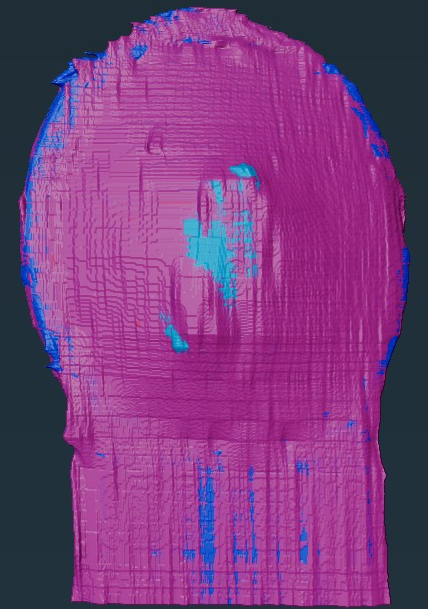
\includegraphics[width=0.5\textwidth]{images/avizo_flats/ins_con.jpg}
	\caption{Volume rendering in Avizo: Insulin control crystal}
 \label{ins_control}
\end{figure}
\begin{figure}
	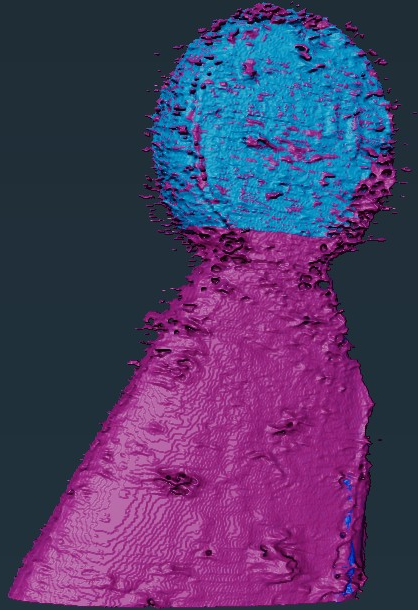
\includegraphics[width=0.5\textwidth]{images/avizo_flats/ins_ls.jpg}
	\caption{Volume rendering in Avizo: Insulin laser-shaped crystal}
 \label{ins_lasershaped}
\end{figure}

\begin{figure}
	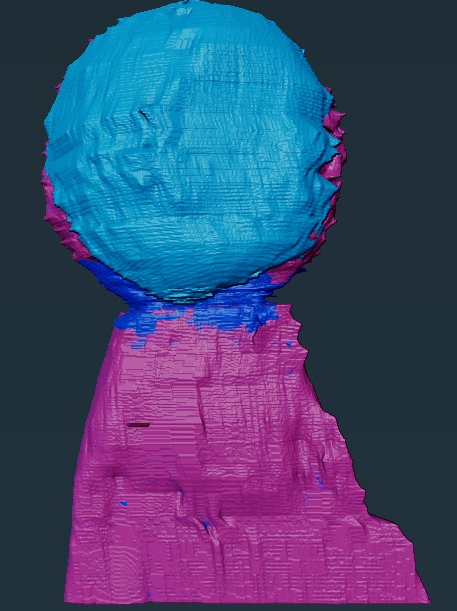
\includegraphics[width=0.5\textwidth]{images/avizo_flats/prot_ls.jpg}
	\caption{Volume rendering in Avizo:}
\end{figure}
\begin{figure}
	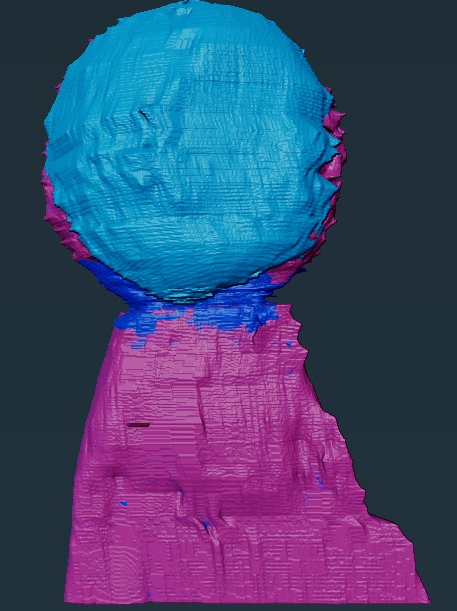
\includegraphics[width=0.5\textwidth]{images/avizo_flats/prot_ls.jpg}
	\caption{Volume rendering in Avizo: Proteinase-K control crystal}
\end{figure}


\onecolumn


\newpage
\section{Tables}

% Please add the following required packages to your document preamble:
% \usepackage{multirow}
% \usepackage{graphicx}
% \usepackage[table,xcdraw]{xcolor}
% Beamer presentation requires \usepackage{colortbl} instead of \usepackage[table,xcdraw]{xcolor}
\begin{table}[h]
\resizebox{\textwidth}{!}{%
\begin{tabular}{|l|l|l|l|l|l|l|}
\hline
\rowcolor[HTML]{C0C0C0} 
\cellcolor[HTML]{C0C0C0}Crystal  & \cellcolor[HTML]{C0C0C0}Energy & Processing symmetry group   & N.o. datasets       & Transmission         & Kappa & Phi \\ \hline
 &
   &
   &
   &
   &
  -25 &
  -100 \\ \cline{6-7} 
 &
   &
   &
   &
   &
  -40 &
  70 \\ \cline{6-7} 
 &
   &
   &
   &
   &
  -35 &
  -70 \\ \cline{6-7} 
 &
   &
  \multirow{-4}{*}{P6122} &
  \multirow{-4}{*}{4} &
  \multirow{-4}{*}{5} &
  0 &
  0 \\ \cline{3-7} 
 &
   &
   &
   &
   &
  -70 &
  0 \\ \cline{6-7} 
 &
   &
   &
   &
   &
  -70 &
  120 \\ \cline{6-7} 
 &
  \multirow{-7}{*}{3.0} &
  \multirow{-3}{*}{P1} &
  \multirow{-3}{*}{3} &
  \multirow{-3}{*}{5} &
  -70 &
  -120 \\ \cline{2-7} 
 &
   &
   &
   &
   &
  0 &
  0 \\ \cline{6-7} 
 &
   &
   &
   &
   &
  -15 &
  100 \\ \cline{6-7} 
 &
   &
   &
   &
   &
  -25 &
  -100 \\ \cline{6-7} 
 &
   &
   &
   &
   &
  -40 &
  70 \\ \cline{6-7} 
 &
   &
  \multirow{-5}{*}{P6122} &
  \multirow{-5}{*}{5} &
  \multirow{-5}{*}{1} &
  -35 &
  -70 \\ \cline{3-7} 
 &
   &
   &
   &
   &
  -70 &
  -120 \\ \cline{6-7} 
 &
   &
   &
   &
   &
  -70 &
  0 \\ \cline{6-7} 
 &
  \multirow{-8}{*}{3.5} &
  \multirow{-3}{*}{P1} &
  \multirow{-3}{*}{3} &
  \multirow{-3}{*}{1} &
  -70 &
  120 \\ \cline{2-7} 
 &
   &
   &
   &
   &
  0 &
  0 \\ \cline{6-7} 
 &
   &
   &
   &
   &
  -15 &
  100 \\ \cline{6-7} 
 &
   &
   &
   &
   &
  -25 &
  -100 \\ \cline{6-7} 
 &
   &
   &
   &
   &
  -40 &
  70 \\ \cline{6-7} 
 &
   &
  \multirow{-5}{*}{P6122} &
  \multirow{-5}{*}{5} &
  \multirow{-5}{*}{1} &
  -35 &
  -70 \\ \cline{3-7} 
 &
   &
   &
   &
   &
  -70 &
  -120 \\ \cline{6-7} 
 &
   &
   &
   &
   &
  -70 &
  0 \\ \cline{6-7} 
\multirow{-23}{*}{Thermolysin 1} & \multirow{-8}{*}{3.8}          & \multirow{-3}{*}{P1}        & \multirow{-3}{*}{3} & \multirow{-3}{*}{1}  & -70   & 120 \\ \hline
 &
   &
   &
   &
   &
  0 &
  0 \\ \cline{6-7} 
 &
   &
   &
   &
   &
  -70 &
  -100 \\ \cline{6-7} 
 &
   &
   &
   &
   &
  -70 &
  0 \\ \cline{6-7} 
                                 & \multirow{-4}{*}{3.0}          & \multirow{-4}{*}{P6122, P1} & \multirow{-4}{*}{4} & \multirow{-4}{*}{20} & -70   & 100 \\ \cline{2-7} 
 &
   &
   &
   &
   &
  0 &
  0 \\ \cline{6-7} 
 &
   &
   &
   &
   &
  -70 &
  -100 \\ \cline{6-7} 
 &
   &
   &
   &
   &
  -70 &
  0 \\ \cline{6-7} 
 &
   &
   &
   &
   &
  -70 &
  100 \\ \cline{6-7} 
\multirow{-9}{*}{Thermolysin 2}  & \multirow{-5}{*}{3.5}          & \multirow{-5}{*}{P6122, P1} & \multirow{-5}{*}{5} & \multirow{-5}{*}{15} & 0     & 0   \\ \hline
\begin{tabular}[c]{@{}l@{}}Insulin 1\\ (laser-shaped)\end{tabular} &
  3.0 &
  I213 &
  1 &
  20 &
  0 &
  0 \\ \hline
\begin{tabular}[c]{@{}l@{}}Insulin 2\\ (control)\end{tabular} &
  3.0 &
  I213 &
  1 &
  15 &
  0 &
  0 \\ \hline
\begin{tabular}[c]{@{}l@{}}Proteinase-K 1\\ (laser-shaped)\end{tabular} &
  3.0 &
  P43212 &
  1 &
  20 &
  0 &
  0 \\ \hline
\begin{tabular}[c]{@{}l@{}}Proteinase-K 2\\ (control)\end{tabular} &
  3.0 &
  P43212 &
  1 &
  20 &
  0 &
  0 \\ \hline
 &
  2.4 &
   &
  2 &
  0.35 &
  0 &
  0 \\ \cline{2-2} \cline{4-7} 
 &
  3.0 &
   &
  3.0 &
  2 &
  0 &
  0 \\ \cline{2-2} \cline{4-7} 
\multirow{-3}{*}{Lysozyme} &
  3.5 &
  \multirow{-3}{*}{P422} &
  3.5 &
  3 &
  0 &
  0 \\ \hline
 &
  3.0 &
   &
  1 &
   &
  0 &
  0 \\ \cline{2-2} \cline{4-7} 
 &
  3.5 &
   &
  1 &
   &
  0 &
  0 \\ \cline{2-2} \cline{4-7} 
 &
  4.0 &
   &
  1 &
   &
  0 &
  0 \\ \cline{2-2} \cline{4-7} 
\multirow{-4}{*}{Thaumatin} &
  4.5 &
  \multirow{-4}{*}{P41212} &
  1 &
   &
  0 &
  0 \\ \hline
\end{tabular}
}
\caption{Diffraction Data Collection Parameters}
\end{table}

%\caption{Diffraction Data Collection Parameters}







% Please add the following required packages to your document preamble:
% \usepackage{booktabs}
% \usepackage{multirow}
% \usepackage{graphicx}
% \usepackage[table,xcdraw]{xcolor}
% Beamer presentation requires \usepackage{colortbl} instead of \usepackage[table,xcdraw]{xcolor}
\begin{table}[]
\resizebox{\textwidth}{!}{%
\begin{tabular}{@{}lllll@{}}
\toprule
Crystal                          & Energy & N.o. datasets & Exposure time (s per 0.2 deg) & Notes                          \\ \midrule
                                 & 3.0    & 4             & 0.35                          &                                \\
                                 & 3.5    & 5             & 0.25                          &                                \\
\multirow{-3}{*}{Thermolysin 1}  & 3.8    & 5             & 0.22                          &                                \\
                                 & 3.0    & 4             & 0.25                          &                                \\
\multirow{-2}{*}{Thermolysin 2}  & 3.5    & 5             & 0.3                           &                                \\
                                 & 3.0    & 1             & 0.3                           &                                \\
\multirow{-2}{*}{Insulin 1}      & 3.5    & 1             & 0.25                          & \multirow{-2}{*}{laser-shaped} \\
                                 & 3.0    & 1             & 0.3                           &                                \\
\multirow{-2}{*}{Insulin 2}      & 3.5    & 1             & 0.25                          & \multirow{-2}{*}{control}      \\
                                 & 3.0    & 1             & 0.3                           &                                \\
\multirow{-2}{*}{Proteinase-K 1} & 3.5    & 1             & 0.25                          & \multirow{-2}{*}{laser-shaped} \\
                                 & 3.0    & 1             & 0.3                           &                                \\
\multirow{-2}{*}{Proteinase-K 2} & 3.5    & 1             & 0.25                          & \multirow{-2}{*}{control}      \\
                                 & 2.4    & 2             & 0.35                          &                                \\
                                 & 3.0    & 2             & 0.3                           &                                \\
\multirow{-3}{*}{Lysozyme}       & 3.5    & 3             & 0.2                           &                                \\
                                 & 3.0    & 1             & 0.35                          &                                \\
                                 & 3.5    & 1             & 0.2                           &                                \\
                                 & 4.0    & 1             & 0.28                          &                                \\
\multirow{-4}{*}{Thaumatin}      & 4.5    & 1             & 0.18                          &       \\
\bottomrule
\end{tabular}%
}

\caption{Tomography Data Collection Parameters used at beamline I23, Diamond Light Source, UK.}
\label{tomo_table}
\end{table}


\newpage
\section{Plots}

\begin{figure}[h]
    \centering
    \begin{tabular}{cc}
    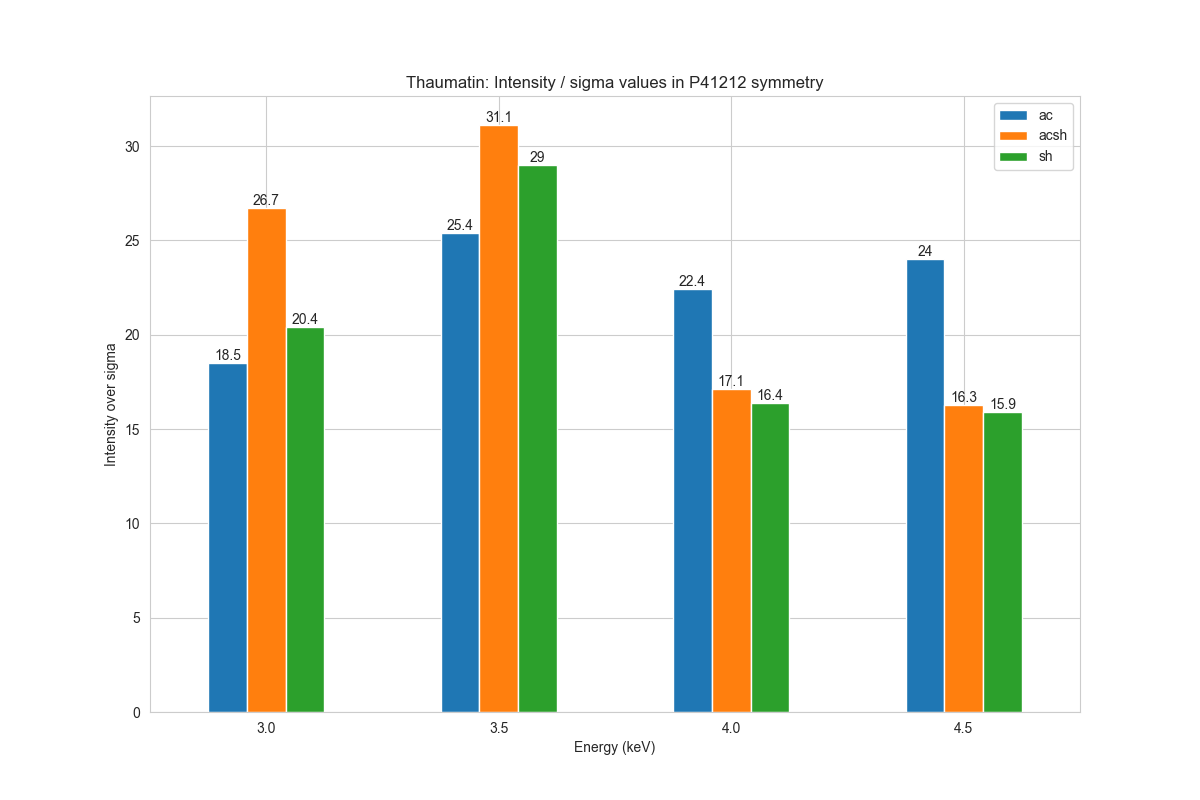
\includegraphics[width = 0.5\textwidth]{plots/exp1/thaum_1/I_over_sigma.png} & 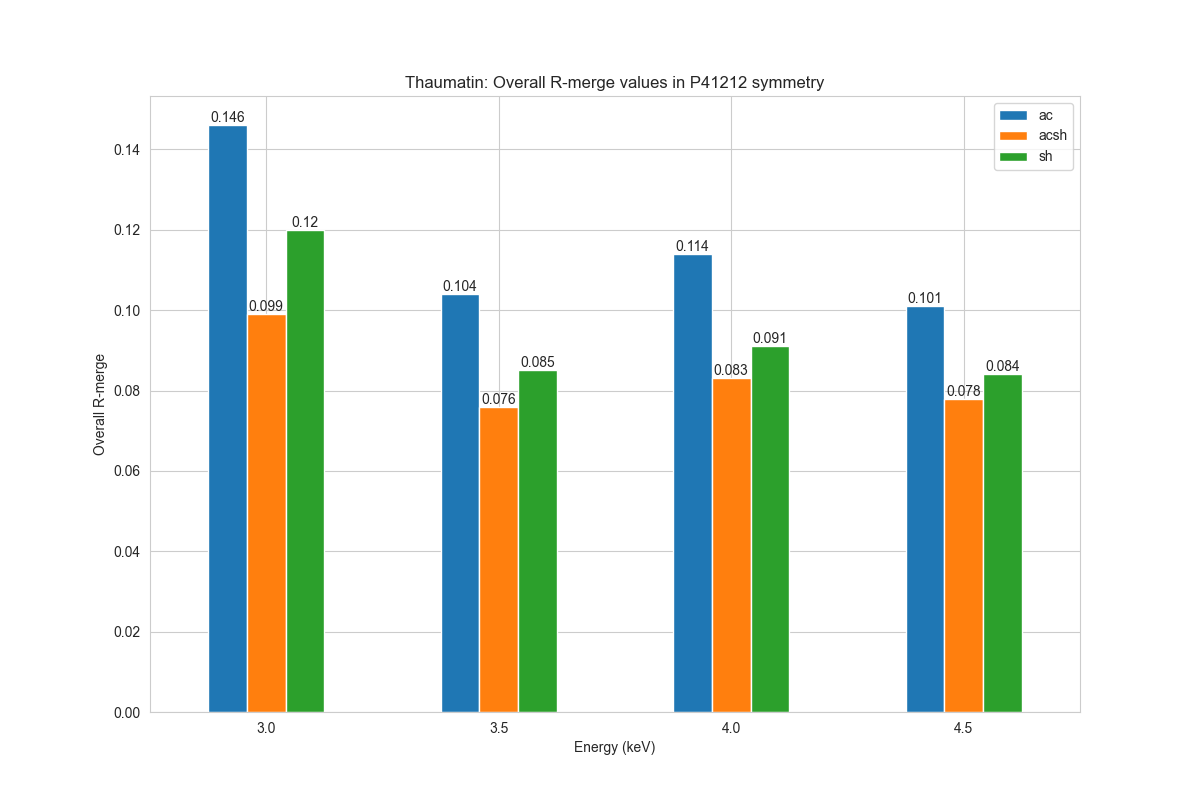
\includegraphics[width = 0.5\textwidth]{plots/exp1/thaum_1/rmerges.png}
    \end{tabular}
    \caption{Caption}
    \label{fig:thaum1_Isig}
\end{figure}